\graphicspath{{notes/3series/asy/}}

\thispagestyle{empty}

\setcounter{section}{13}
\section{Series}\label{sec:series}


What should be meant by the following expression?
\[\sum_{n=1}^\infty \frac 1{n^2}=1+\frac 14+\frac 19+\frac 1{16}+\cdots\]
The \emph{$\infty$}-symbol in the summation should lead you to suspect a role for \emph{limits\ldots}

\begin{defn}{}{}
	Define the \emph{$n\th$ partial sum} $s_n$ of a sequence $(a_n)_{n=m}^\infty$ via
	\[s_n:=\smash{\sum_{k=m}^n}a_k=a_m+a_{m+1}+\cdots+a_n\]
	\begin{itemize}
	  \item The \emph{(infinite) series}\footnotemark{} $\smash[b]{\sum\limits_{n=m}^\infty a_n}$ is the limit $\lim s_n$ of the sequence $(s_n)$ of partial sums.
	  \item A series \emph{converges, s to $\pm\infty$} or \emph{diverges by oscillation} as does the sequence $(s_n)$.
	  \item $\sum a_n$ \emph{converges absolutely} if $\sum\nm{a_n}$ converges.
	  \item $\sum a_n$ \emph{converges conditionally} if it converges but not absolutely ($\sum \nm{a_n}$ diverges to $\infty$).
	\end{itemize}
\end{defn}

\footnotetext{It is common to denote a series $\sum a_n$ if the initial term is understood (typically $a_0$ or $a_1$), or is irrelevant to the situation.}

%A series of non-negative terms can only converge (absolutely) or diverge to $+\infty$. 
To return to our motivating example,
\[
	\sum_{n=1}^\infty \frac 1{n^2}=\lim s_n\quad\text{where}\quad s_n=\sum\limits_{k=1}^n \frac 1{k^2}=1+\frac 14+\cdots+\frac 1{n^2}
\]
We don't (yet) know whether the series converges or diverges to $\infty$\ldots

\begin{thm}{Basic Series Laws}{basicserieslaws}
	Infinite series behave nicely with respect to addition and scalar multiplication. For instance:
	\begin{enumerate}
	  \item If $\sum a_n$ is convergent and $k$ is constant, then $\sum ka_n=k\sum a_n$ is convergent.
	  \item If $\sum a_n$ and $\sum b_n$ are convergent, then $\sum(a_n\pm b_n)=\sum a_n\pm\sum b_n$ are also convergent.
	  \item If $\sum a_n=\infty$ and $k>0$, then $\sum ka_n=\infty$.
	  \item If $\sum a_n=\infty$ and $\sum b_n$ converges, then $\sum(a_n+b_n)=\infty$.
	\end{enumerate}
\end{thm}

\begin{proof}
	Simply apply the limit/divergence laws to the sequence of partial sums. E.g.{} for 1,
	\[
	  \sum ka_n = \lim_{n\to\infty}\sum_{j=m}^nka_j \overset{\text{finite}}{\overset{\text{sum}}{=}} \lim_{n\to\infty}k\sum_{j=m}^na_j \overset{\text{limit}}{\overset{\text{laws}}{=}} k\lim_{n\to\infty}\sum_{j=m}^na_j =k\sum a_n
	\]
	The others may be proved similarly.
\end{proof}


Note that series do not behave nicely with respect to multiplication (see also Exercise \ref{exs:seriesmult}):
\[
	a_1b_1+a_2b_2+\cdots =\sum a_nb_n\neq \bigl(\sum a_n\bigr)\bigl(\sum b_n\bigr) =\bigl(a_1+a_2+\cdots\bigr)\bigl(b_1+b_2+\cdots\bigr)
\]

\goodbreak


\boldsubsection{Series which may be evaluated exactly}

Our major goal is to develop techniques for answering the binary question, ``Does $\sum a_n$ converge?'' Even when the answer is \emph{yes,} a precise computation of the limit is usually beyond us. However, our techniques (the upcoming \emph{series tests}) will typically rely on comparing $\sum a_n$ to a `standard' series whose properties are completely understood. You have met two such series in elementary calculus.

\begin{defn}{Geometric series}{}
	A sequence $(a_n)$ is \emph{geometric} if the ratio of successive terms is constant: $a_n=ba^n$ for some constants $a,b$. A \emph{geometric series} is the sum of a geometric sequence. 
\end{defn}

The computation of the sequence of partial sums should be familiar (for simplicity assume $b=1$)
\[(1-a)s_n=\bigl(a^m+\textcolor{blue}{a^{m+1}+\cdots+a^n}\bigr)-\bigl(\textcolor{blue}{a^{m+1}+a^{m+2}+\cdots +a^n}+a^{n+1}\bigr) =a^m-a^{n+1}\]
from which we quickly conclude:

\begin{thm}{}{}
	If $a$ is constant, then
	\[s_n=\sum_{k=m}^n a^k=\begin{cases}
	\dfrac{a^m-a^{n+1}}{1-a}&\text{if }a\neq 1\\
	n+1-m&\text{if }a=1
	\end{cases}\implies \sum_{n=m}^\infty a^n\begin{cases}
	\text{converges to }\dfrac{a^m}{1-a}&\text{if }\nm{a}<1\\
	\text{diverges to $\infty$}&\text{if }a\ge 1\\
	\text{diverges by oscillation}&\text{if }a\le -1
	\end{cases}\]
	In particular, $\sum a^n$ converges absolutely if $\nm a<1$ and diverges otherwise. 
\end{thm}


\begin{examples}{}{}
	\exstart $\displaystyle \sum_{n=-1}^\infty 2\left(-\frac 45\right)^n= 2\frac{\left(-\frac 45\right)^{-1}}{1+\frac 45} =-\frac 52\cdot\frac 59= -\frac{25}{18}$
	\begin{enumerate}\setcounter{enumi}{1}
	  \item Consider the series $\sum a_n=\smash[b]{\sum\limits_{n=3}^\infty} \left(\frac 25\right)^n +2^n$. If this were convergent, then
		\[\sum 2^n=\sum a_n-\sum\left(\frac 25\right)^n\]
		would converge (Theorem \ref{thm:basicserieslaws}); a contradiction.
	\end{enumerate}
\end{examples}


\boldinline{Telescoping series}

A rarer type of series can be evaluated using the algebra of partial fractions.

\begin{example}{}{}
	To compute $\sum\limits_{n=1}^\infty\frac 1{n(n+1)}$, first  observe that
	\[s_n=\sum_{k=1}^n\frac 1{k(k+1)} =\sum_{k=1}^n\frac 1k-\frac 1{k+1} =\frac 11\textcolor{blue}{-\frac 12+\frac 12-\frac 13+\cdots+\frac 1n}-\frac 1{n+1}=1-\frac 1{n+1}\]
	It follows that
	\[\sum_{n=1}^\infty\frac 1{n(n+1)}=\lim \left(1-\frac 1{n+1}\right)=1\]
	Similar arguments can be made for other series such as $\sum\frac 1{n(n+2)}$.
\end{example}

\goodbreak


\boldsubsubsection{The Cauchy Criterion}

The starting point for general series convergence uses Cauchy completeness.

\begin{example}{}{}
	Consider again the series $\sum\frac 1{n^2}$. We show that the sequence of partial sums $(s_n)$ is Cauchy. Let $\epsilon>0$ be given and let $N=\frac 1\epsilon$. Then,
	\begin{align*}
	m>n>N\implies \nm{s_m-s_n}&=\sum_{k=n+1}^m\frac 1{k^2}<\sum_{k=n+1}^m\frac 1{k(k-1)} =\sum_{k=n+1}^m\frac 1{k-1}-\frac 1k\\
	&=\frac 1n-\frac 1m<\frac 1N=\epsilon
	\end{align*}
	where we follow the telescoping series approach to cancel most terms. By Cauchy completeness (Theorem \ref{thm:convcauchy}), $(s_n)$ converges and we conclude
	\[
		\tcbhighmath{\text{The series $\displaystyle \sum\frac 1{n^2}$ is convergent}}
	\]
	Computing the value of this series rigorously is significantly harder, though a sketch argument for why $\sum\frac 1{n^2}=\frac{\pi^2}6$ is in Exercise \ref{exs:eulersum}.
\end{example}

\begin{thm}{Cauchy Criterion for Series}{}
	A series $\sum a_n$ converges if and only if
	\[
		\forall\epsilon>0,\ \exists N\text{ such that }m\ge n>N\implies\nm{s_m-s_{n-1}}=\nm{\sum_{k=n}^ma_k}<\epsilon
	\]
\end{thm}

In the previous example we essentially verified the Cauchy criterion for the series $\sum\frac 1{n^2}$.

\begin{proof}
	Let $(s_n)$ be the sequence of partial sums. Then
	\begin{align*}
		\sum a_n\text{ converges}&\iff (s_n)\text{ converges} \iff (s_n)\text{ is Cauchy} \tag{Thm \ref{thm:convcauchy}}\\
		&\iff \Bigl(\forall\epsilon>0,\ \exists N\text{ such that }m>n>N\implies\nm{s_m-s_n}<\epsilon\Bigr)
	\end{align*}
	To finish, simply replace $n$ with $n-1$. 
\end{proof}

\begin{example}{}{harmonic}
	Assume, for contradiction, that the \emph{harmonic series} $\sum\frac 1n$ converges. Now take $\epsilon=\frac 12$ in the Cauchy criterion:
	\[\exists N\text{ such that }m\ge n>N\implies \nm{\sum_{k=n}^{m}\frac 1k}<\frac 12\]
	However, taking $m=2(n-1)\ge n$ (true since $n>N\ge 1$) results in a contradiction: 
	\[\frac 12>\nm{\sum_{k=n}^{m}\frac 1k}=\nm{\frac 1n+\cdots+\frac 1m}\ge \frac{m-(n-1)}{m}=1-\frac{n-1}m=\frac 12\]
	We conclude that the harmonic series diverges to $\infty$.
\end{example}

\goodbreak


\boldsubsubsection{The Series Tests}

For the remainder of this section we develop several standard tests for the convergence/divergence of an infinite series: the divergence, comparison, root and ratio tests. The first of these follow quickly from the Cauchy criterion.

\begin{thm}{Divergence/$n\th$-term test}{}
	If $\lim a_n\neq 0$ then $\sum a_n$ is divergent.
\end{thm}

\begin{proof}
	We prove the contrapositive. Suppose $\sum a_n$ is convergent, let $\epsilon>0$ be given and take $m=n$ in the Cauchy criterion. Then
	\[\exists N\text{ such that }n>N\implies\nm{a_n}<\epsilon\]
	Otherwise said, $\lim a_n=0$.
\end{proof}


\begin{examples}{}{}
	\exstart The series $\sum\sin(\frac{n\pi}9)$ diverges.
	\begin{enumerate}\setcounter{enumi}{1} 
	  \item The divergence test tells us that the geometric series $\sum a^n$ diverges whenever $\nm a\ge 1$. We still need our earlier analysis for when $\nm a<1$.
	  \item The \emph{converse of the $n^\text{th}$-term test is false!} For the canonical example, consider the \emph{divergent} harmonic series $\sum \frac 1n$ (Example \ref{ex:harmonic}, even though $\lim\frac 1n=0$.
	\end{enumerate}
\end{examples}


\begin{thm}{Comparison test}{}
\exstart Let $\sum b_n$ be a convergent series of non-negative terms and assume $\nm{a_n}\le b_n$ for all (large $n$). Then both $\sum b_n$ and $\sum \nm{b_n}$ are convergent.
	\begin{enumerate}\setcounter{enumi}{1}
	  \item If $\sum a_n=\infty$ and $a_n\le b_n$ for all (large) $n$, then $\sum b_n=\infty$.
	\end{enumerate}
\end{thm}

\begin{proof}
Suppose ``large $n$" means $n>M$. 
	\begin{enumerate}
	  \item Let $\epsilon>0$ be given. Then $\exists N\ge M$ such that
		\[m\ge n>N\implies\nm{\sum_{k=n}^ma_k}\overset{\triangle}{\le}\sum_{k=n}^m\nm{a_k}\le\sum_{k=n}^mb_k<\epsilon\]
		\item The $n\th$ partial sum of $\sum b_n$ is
		\[\sum_{k=M}^nb_k\ge \sum_{k=M}^na_k\to+\infty\tag*{\qedhere}\]
	\end{enumerate}
\end{proof}

\begin{cor}{}{compest}
	\exstart Take $\nm{a_n}=b_n$ in part 1 to see that $\sum\nm{a_n}$ converges $\implies \sum a_n$ converges. Thus absolute convergence implies convergence.
	\begin{enumerate}\setcounter{enumi}{1}
	  \item If $\sum b_n$ is a convergent series of non-negative terms and $\nm{a_n}\le b_n$ for \underline{all} $n$, then
	  \[\sum a_n\le \sum\nm{a_n}\le \sum b_n\]
	\end{enumerate}
\end{cor}

\goodbreak


\begin{examples}{}{compexs}
	\exstart Since $\frac{2n+1}{(n+2)3^n}\le 2\cdot 3^{-n}$ and the geometric series $\sum 2\cdot 3^{-n}$ converges, we see that the resulting series converges (absolutely), to some value
	\[\sum_{n=0}^\infty\frac{2n+1}{(n+2)3^n}\le 2\sum_{n=0}^\infty 3^{-n}=\frac 2{1-\frac 13}=3 \]
	
	\begin{enumerate}\setcounter{enumi}{1}
	  \item One can usually find a sensible series to compare with just by thinking about how $a_n$ behaves when $n$ is very large. For instance, $a_n=\smash[b]{\frac{(n^2+1)^{1/2}}{(1+\sqrt n)^4}}$ behaves like $\smash[b]{\frac{n}{n^2}=\frac 1{n}}$ and we see that
	  \[a_n>\frac n{(1+\sqrt n)^4}>\frac n{(2\sqrt n)^4}=\frac 1{16n}\]
	  Comparison with $\frac 1{16}\sum \frac 1n$ shows that $\sum a_n$ diverges to $\infty$.
	  
		\item Since $\ln n<n\implies\frac 1{\ln n}>\frac 1n$, we see that $\sum \frac 1{\ln n}$ diverges to $\infty$ by comparison with $\sum\frac 1n$.
		
	  \item $\sum\frac{\sin n}{n^2}$ converges absolutely by comparison to $\sum\frac 1{n^2}$. Corollary \ref{cor:compest} gives an estimation for the value of the series, though it is not accurate! The $n^\text{th}$ partial sums satisfy
		\begin{gather*}
		\textcolor{red}{\sum_{n=1}^\infty\frac{\sin n}{n^2}} \le \textcolor{blue}{\sum_{n=1}^\infty \frac{\nm{\sin n}}{n^2}} \le \sum_{n=1}^\infty\frac 1{n^2} = \frac{\pi^2}6 \tag{approximately $\textcolor{red}{1.014}\le \textcolor{blue}{1.280} \le 1.645$}
		\end{gather*}
		
	  %\item $\sum\frac{(-1)^{n+1}}{n^2}$ converges absolutely by comparison with $\sum\frac 1{n^2}$.
	  
	  
	  \item\label{ex:altharmonic1} The \emph{alternating harmonic series} $\sum\limits_{n=1}^\infty\frac{(-1)^{n+1}}n$ converges via a sneaky comparison.\par
	   Consider the series $\smash{t=\sum\limits_{n=1}^\infty \frac 1{2n(2n-1)}}$ which converges by comparison with $\smash{\sum\frac 1{4(n-1)^2}}$. Its $n\th$ partial sum is
	  \[t_n=\sum_{k=1}^{n}\frac 1{2k(2k-1)}=\sum_{k=1}^n\left[\frac 1{2k-1}-\frac 1{2k}\right]\]
	  which is the \emph{even} partial sum of the alternating harmonic series $s_{2n}=\sum_{m=1}^{2n}\frac{(-1)^{m+1}}m$.\par
	  Take limits of $s_{2n+1}=s_{2n}+\frac 1{2n+1}$, we see that $\lim s_{2n+1}=t$ from which $\lim s_n=t$. Since the harmonic series $\sum\frac 1n$ diverges (Example \ref{ex:harmonic}), we conclude that the alternating harmonic series converges conditionally. We will revisit this discussion in the next section.
	  
	  
	% 	\item $\displaystyle\sum\left(1-\frac 1n\right)^{n^2}$ converges by comparison with the geometric series $\displaystyle\sum 2^{-n}$: since
	% 	\[\left(1-\frac 1n\right)^n\xrightarrow[n\to\infty]{}e^{-1}<\frac 12\]
	% 	we see that, for all large\footnote{Strictly $\exists N$ such that $n>N\implies \left(1-\frac 1n\right)^n<\frac 12$. In fact this is true for all positive $n$, for the sequence $\left(1-\frac 1n\right)^n$ is monotone-up\ldots} $n$,
	% 	\[\left(1-\frac 1n\right)^n<\frac 12\implies \left(1-\frac 1n\right)^{n^2}\le 2^{-n}\]
	
	
	
	
		\item\label{ex:root5} $\sum\left(\frac n{n+1}\right)^{n^2}$ converges by comparison with the geometric series $\sum 2^{-n}$. To see this, note that
		\[\left(\frac n{n+1}\right)^n=\frac{n+1}n\left(1-\frac 1{n+1}\right)^{n+1}\xrightarrow[n\to\infty]{}e^{-1}<\frac 12\]
		from which we see that, for all large $n$,
		\[\left(\frac n{n+1}\right)^n<\frac 12\implies \left(\frac n{n+1}\right)^{n^2}< 2^{-n}\]
		In fact (compare Exercise \ref*{sec:monocauchy}.\ref{exs:edefn}), $\left(\frac n{n+1}\right)^n$ is monotone-down, whence $e^{-1}\le \left(\frac n{n+1}\right)^n\le \frac 12$ and
		\[0.58198\approx\frac 1{e-1}=\frac{e^{-1}}{1-e^{-1}}=\sum_{n=1}^\infty e^{-n}\le \sum_{n=1}^\infty\left(\frac n{n+1}\right)^{n^2}\le \sum_{n=1}^\infty 2^{-n}=\frac{1/2}{1-1/2}=1\]
		A computer estimate yields $\sum\limits_{n=1}^\infty\left(\frac n{n+1}\right)^{n^2}\approx 0.8174$.
	\end{enumerate}
\end{examples}


%The comparison test is very powerful, though it sometimes requires significant creativity to apply. Note also that, at best, it can only provide an \emph{estimate} for the value of a convergent series; in practice such estimates can often be bettered simply by summing the first few terms with a calculator!

\goodbreak

Our final two tests in this section are less powerful, but have the advantage of being easier to use. %Both are special cases of previous tests: their convergence versions depend on the comparison test and their divergence versions on the $n\th$-term test.


\begin{thm}{Root test}{}
Let $\limsup\nm{a_n}^{1/n}=L$.
\begin{enumerate}
	\item If $L<1$, then $\sum a_n$ converges absolutely.
	\item If $L>1$, then $\sum a_n$ diverges.
\end{enumerate}
If $L=1$, then no conclusion can be drawn.
\end{thm}

We defer the proof until after seeing some examples.

\begin{cor}{Ratio test}{}
Suppose $(a_n)$ is a sequence of non-zero terms.
\begin{enumerate}
	\item If $\smash{\limsup\nm{\frac{a_{n+1}}{a_n}}<1}$, then $\sum a_n$ converges absolutely 
	\item If $\liminf\nm{\frac{a_{n+1}}{a_n}}>1$, then $\sum a_n$ diverges
\end{enumerate}
\end{cor}

\begin{proof}
	This follows directly from the root test and Theorem \ref{thm:rootratio}:
	\[\liminf\nm{\frac{a_{n+1}}{a_n}}\le\liminf\nm{a_n}^{1/n}\le\limsup\nm{a_n}^{1/n}\le \limsup\nm{\frac{a_{n+1}}{a_n}}\tag*{\qedhere}\]
\end{proof}

The versions of these tests familiar from elementary calculus are the special cases when
\[
	L=\lim\nm{a_n}^{1/n}=\lim\nm{\frac{a_{n+1}}{a_n}}
\]
Our versions are more general since these limits are \emph{not guaranteed to exist.}

\begin{examples}{}{}
\exstart The ratio test is particularly useful for series involving \emph{factorials} and \emph{exponentials.}
\begin{enumerate}\setcounter{enumi}{1}
	\item[]\begin{enumerate}
	  \item $\sum\frac{n^4}{2^n}$ converges: just observe that $\lim\nm{\frac{a_{n+1}}{a_n}}=\lim\frac{(n+1)^4}{2n^4}=\frac 12<1$.
		\item $\sum\frac{n!}{2^n}$ diverges: in this case $\lim\nm{\frac{a_{n+1}}{a_n}} =\lim\frac{(n+1)!}{2n!}=\lim \frac{n+1}2=\infty$.
	\end{enumerate}
	
	\item Both tests are inconclusive for rational sequences: if $a_n=\frac{b_n}{c_n}$ where $b_n,c_n$ are polynomials, then
	\[\lim\nm{\frac{a_{n+1}}{a_n}}=1=\lim\nm{a_n}^{1/n}\]
	For example,
	\[\sum\frac{n+5}{n^2}\rightsquigarrow \lim\nm{\frac{a_{n+1}}{a_n}} =\lim \frac{(n+6)n^2}{(n+5)(n+1)^2}=1\]
	In fact this example is divergent by comparison with the harmonic series $\sum \frac 1n$.
	
	
	\item Recall Example \ref*{ex:compexs}.\ref{ex:root5}: our use of the comparison test was really the root test in disguise
	\[a_n=\left(\frac n{n+1}\right)^{n^2}\implies \lim\nm{a_n}^{1/n}= \lim\left(\frac n{n+1}\right)^{n}=e^{-1}<1 \implies \sum a_n\text{ converges}\]
	In this case the root test was much easier to apply!
	
	\goodbreak
	
	\item The ratio test is the weakest test thus far; certainly it does not apply if any of the terms $a_n$ are zero! For a more subtle example, consider:
	\[a_n=\begin{cases}
	2^{-n}&\text{ if $n$ is even}\\
	3^{-n}&\text{ if $n$ is odd}
	\end{cases}\]
	First we try applying the ratio test:
	\[\frac{a_{n+1}}{a_n}=\begin{cases}
	\frac 13\left(\frac 23\right)^{n}&\text{ if $n$ is even}\\
	\frac 12\left(\frac 32\right)^{n}&\text{ if $n$ is odd}
	\end{cases}\quad\implies \liminf\nm{\frac{a_{n+1}}{a_n}}=0,\quad \limsup\nm{\frac{a_{n+1}}{a_n}}=\infty\]
	The ratio test is therefore inconclusive.	However
	\[\nm{a_n}^{1/n}=\begin{cases}
	\frac 12&\text{ if $n$ is even}\\
	\frac 13&\text{ if $n$ is odd}
	\end{cases}\implies \limsup\nm{a_n}^{1/n}=\frac 12<1\]
	By the root test, the series $\sum a_n$ converges.
	We need not even have used the root test: $\sum a_n$ converges by comparison with $\sum 2^{-n}$!
	%\footnote{We can actually be more precise: using the basic series laws and the fact that the even and odd terms form convergent geometric series,
	%\[\sum_{n=0}^\infty a_n=\sum_{k=0}^\infty 2^{-2k}+3^{-2k-1}=\frac 1{1-1/4}+\frac 13\cdot \frac 1{1-1/9}=\frac{11}8\]}
\end{enumerate}
\end{examples}




\begin{proof}[Proof of the Root Test]
\begin{enumerate}
	\item Suppose $\limsup\nm{a_n}^{1/n}=L<1$. Recall that $v_N=\sup\{\nm{a_n}^{1/n}:n>N\}$ defines a \emph{monotone-down} sequence converging to $L$. Choose any $\epsilon>0$ such that $L+\epsilon<1$ (say $\epsilon=\frac{1-L}2$) to see that
	\[\exists N\text{ such that }v_N-L<\epsilon \]
	But then
	\[n>N\implies\nm{a_n}^{1/n}-L<\epsilon\implies \nm{a_n}<(L+\epsilon)^n\]
	$\sum\nm{a_n}$ therefore converges by comparison with the geometric series $\sum(L+\epsilon)^n$.
	
	\item If $L>1$ then there exists some subsequence $(a_{n_k})$ such that $\nm{a_{n_k}}^{1/n_k}\to L>1$. In particular, infinitely many terms of this subsequence must be greater than 1. Clearly $a_n$ does not converge to zero whence the series diverges by the $n^\text{th}$ term test.\hfill\qedhere
\end{enumerate}
\end{proof}

\boldinline{Summary}
The logical flow of the tests in this section is as follows:
\[\xymatrix{ \text{(divergence tests)} & & n^\text{th} \text{ term} \ar@{=>}[r] & \text{Root} \ar@{=>}[r] & \text{Ratio} \\
\text{(testing both)} & \text{Definition of }\sum a_n \ar@{<=>}[r] & \text{ Cauchy Criterion} \ar@{=>}[u] \ar@{=>}[r] & \text{Comparison} \ar@{=>}[d]& \\
\text{(convergence tests)} &&& \text{Root} \ar@{=>}[r] & \text{Ratio}
}\] 
The ratio test is typically the easiest to use, but the least powerful. Every series which converges by the ratio test can be seen to converge by the root and comparison tests, etc. If a series diverges by the ratio test, then it in fact diverges by the $n^\text{th}$ term test.

\clearpage

\begin{exercisessec}{}{}
	\exstart %[2+4.]
	Determine which of the following sequences converge. Justify your answers.\vspace{-2pt}
	\begin{enumerate}\setcounter{enumi}{1}
    \item[]\begin{enumerate}
			\item \makebox[100pt][l]{$\sum\frac{n-1}{n^2}$ \hfill (b)} \  \makebox[100pt][l]{$\sum (-1)^n$\hfill (c)} \ \makebox[100pt][l]{$\sum\frac{3^n}{n^3}$ \hfill (d)} \ $\sum\frac{n^3}{3^n}$
			\setcounter{enumii}{4}
			\item \makebox[100pt][l]{$\sum\frac{n^2}{n!}$ \hfill (f)} \  \makebox[100pt][l]{$\sum\frac 1{n^n}$\hfill (g)} \ \makebox[100pt][l]{$\sum\frac{n}{2^n}$ \hfill (h)} \ $\sum\frac{n!}{n^n}$
			\setcounter{enumii}{8}
			\item \makebox[100pt][l]{$\sum\limits_{n=2}^\infty\frac 1{\bigl[n+(-1)^n\bigr]^2}$ \hfill (j)} \  \makebox[100pt][l]{$\sum \bigl[\sqrt{n+1}-\sqrt n\bigr]$}
		\end{enumerate}
		
  
	   \item%[8.]
	   Let $\sum a_n$ and $\sum b_n$ be convergent series of non-negative terms. Prove that $\sum \sqrt{a_nb_n}$ converges.\par
	  	(\emph{Hint: start by showing that $\sqrt{a_nb_n}\le a_n+b_n$})
	  
  
  
	  \item%[6.] + variation
	  \label{exs:seriesmult}
	  \begin{enumerate}
	    \item If $\sum a_n$ converges absolutely, prove that $\sum a_n^2$ converges.
	    \item More generally, if $\sum\nm{a_n}$ converges and $(b_n)$ is a bounded sequence, prove that $\sum a_nb_n$ converges absolutely.
	    %\item Are parts (a), (b) true if $\sum a_n$ converges conditionally? Explain.
	  \end{enumerate}
	  
	  
	  \item%[10.]
		Find a series $\sum a_n$ which diverges by the root test but for which the ratio test is inconclusive.
	  
	  \item%[12.]
	  (Hard) \ Let $(a_n)$ be a sequence such that $\liminf\nm{a_n}=0$. Prove that there is a subsequence $(a_{n_k})$ such that $\sum a_{n_k}$ converges.\par
	  (\emph{Hint: Try to construct a subsequence which converges to zero faster than $\frac 1{k^2}$.}
	  
	  \item%[14.]
	  Prove that the harmonic series $\sum\frac 1n$ diverges by comparing with the series $\sum a_n$, where
	  \[(a_n)=\textstyle\left(1,\frac 12,\frac 14,\frac 14,\frac 18,\frac 18,\frac 18,\frac 18,\frac 1{16},\frac 1{16},\frac 1{16},\frac 1{16},\frac 1{16},\frac 1{16},\frac 1{16},\frac 1{16},\frac 1{32},\frac 1{32},\ldots\right)\]
	  
	  
	  \item Suppose $b_n\le a_n$ for all $n$ and that $\sum b_n$ and $\sum a_n$ converge. Prove that $\sum b_n\le \sum a_n$.\par
	  (\emph{This also proves part 2 of Corollary \ref{cor:compest}})

	
		\item Use the basic series laws to find the values of $\sum \frac 1{(2n)^2}$, $\sum\frac 1{(2n+1)^2}$ and $\sum\frac{(-1)^{n+1}}{n^2}$.

	
	\item The \emph{limit comparison test} states:
  \begin{quote}
  	Suppose $\sum a_n$, $\sum b_n$ are series of positive terms and that $L=\lim\frac{a_n}{b_n}\in(0,\infty)$. Then the series have the same convergence status (both converge or both diverge to $\infty$).
  \end{quote}
  \begin{enumerate}
%     \item Determine whether the series $\displaystyle \sum_{n=0}^\infty\frac{(3n^2+4)\sqrt n}{2n^4-1}$ converges or diverges.\marks{5}
    \item Use the limit comparison test with $b_n=\frac 1{n^2}$ to show that the series $\sum\frac 1n\ln\left(1+\frac 1n\right)$ converges.\par
    (\emph{Hint: Recall that $e=\lim\left(1+\frac 1n\right)^n$})
    	
    \item Prove the limit comparison test.\par
    (\emph{Hint: first show that $\frac L2<\frac{a_n}{b_n}<\frac{3L}2$ for large $n$})
    	
    \item What can you say about the series $\sum a_n$ and $\sum b_n$ if $L=0$ or $L=\infty$? Explain.
  \end{enumerate}
  
  
	  
	  \item\label{exs:eulersum} Euler asserted that the sine function, written as an infinite polynomial in the form of a Maclaurin series, could also be expressed as an infinite product,
	  \[\sin x =\sum_{n=0}^\infty \frac{(-1)^n}{(2n+1)!}x^{2n+1} =x\left(1-\frac{x^2}{\pi^2}\right)\left(1-\frac{x^2}{4\pi^2}\right)\left(1-\frac{x^2}{9\pi^2}\right)\cdots \]
	  By considering the solutions to $\sin x=0$, give some weight to Euler's claim. By comparing coefficients in these expressions, deduce the fact $\sum \frac 1{n^2}=\frac{\pi^2}6$.\par
	  (\emph{As we've presented it, this argument is non-rigorous!})
	\end{enumerate}
\end{exercisessec}


\clearpage

\section{The Integral and Alternating Series Tests}

In this section we develop two further standalone series tests, both with narrower applications than our previous tests.\smallbreak


The first a little out of place given that it requires (improper) integration.\footnote{Which in turn requires limits of functions: $\int_1^\infty f(x)\,\dx:=\lim\limits_{b\to\infty}\int_1^bf(x)\,\dx$. Even though we haven't developed these concepts, the relevant computations should be familiar from elementary calculus.} 

\begin{thm}[lower separated=false, sidebyside, sidebyside align=top seam, sidebyside gap=0pt, righthand width=0.4\linewidth]{Integral test}{}
	Let $a_n=f(n)$, where $f$ is non-negative, non-increasing and integrable on $[1,\infty)$. Then
	\[\sum_{n=1}^\infty a_n\ \text{converges} \iff \int_1^\infty f(x)\,\dx\ \text{converges}\]
	in which case
	\[\int_1^\infty f(x)\,\dx\le\sum_{n=1}^\infty a_n\le a_1+\int_1^\infty f(x)\,\dx\]
	The statement is easily modified if the initial term is $a_m$.
% 	Regardless of convergence, the $n\th$ partial sum satisfies:
% 	\[\int_1^{n+1}f(x)\,\dx\le s_n\le a_1+\int_1^nf(x)\,\dx \tag*{($\ast$)}\]
% 	\[
% 		s_n=\begin{cases}
% 			\textcolor{blue}{\sum\limits_{k=1}^n a_k}\le\int_1^{n+1}f(x)\,\dx\\
% 			a_1+\textcolor{Green}{\sum\limits_{k=2}^na_k}\ge a_1+\int_1^nf(x)\,\dx
% 		\end{cases}
% 	\]
	\tcblower
	\flushright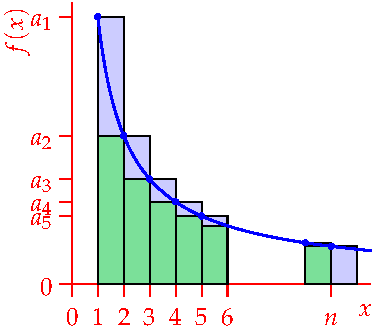
\includegraphics[scale=0.9]{integraltest}
\end{thm}

\begin{proof}
	We need only interpret the picture:
	\[\int_1^{n+1}f(x)\,\dx\le\textcolor{blue}{\sum_{k=1}^n a_k} =s_n= a_1+\textcolor{Green}{\sum_{k=2}^na_k}\le a_1+\int_1^nf(x)\,\dx \tag*{($\ast$)}\]
	Taking limits gives the result.
\end{proof}


Even for divergent sums, $(\ast)$ allows us to estimate $s_n$ and analyze its rate of growth. For greater accuracy, explicitly evaluate the first few terms and use a modified integral test to estimate the remainder.\smallbreak
The big application of the integral test is a complete description of the convergence status of $p$-series, another useful collection of series to which others may be compared.

\begin{cor}{$p$-series}{pseries}
 	Let $p>0$. The series $\sum\frac 1{n^p}$ converges if and only if $p>1$.
\end{cor}

\goodbreak


\begin{examples}{}{inttestex}
	\exstart $\smash{\sum
	%\limits_{n=1}^\infty 
	\frac 1{n^3}}$ converges (it is a $p$-series with $p>1$). For a simple estimate, observe that
	\[
		\int_1^\infty\frac 1{x^3}\,\dx =\lim_{b\to\infty}\left[-\frac 12x^{-2}\right]_1^b =\frac 12 \implies \frac 12\le \sum_{n=1}^\infty\frac 1{n^3}\le\frac 32
	\]
	This is a poor estimate, especially the lower bound. For a quick improvement, we could explicitly evaluate the first term and re-run the test starting at $n=2$:
	\[
		1+\int_{2}^\infty\frac 1{x^3}\,\dx \le\sum_{n=1}^\infty \frac 1{n^3} \le 1+\frac 18 +\int_{2}^\infty\frac 1{x^3}\,\dx
		\implies 1+\frac 18\le \sum_{n=1}^\infty \frac 1{n^3}\le 1+\frac 14
	\]
	If greater accuracy is required, more terms can be explicitly evaluated.
	
	\goodbreak
	
\begin{enumerate}\setcounter{enumi}{1}	
% 	\item The function $f(x)=x^{-2}\sin(x^{-1})$ is positive and decreasing. Moreover, with the substitution $u=x^{-1}$, we have a convergent integral:
% 	\[\int_1^\infty f(x)\,\dx =\int_0^1 \sin u\,\du=1-\cos(1)\]
% 	It follows that the series $\displaystyle \sum_{n=1}^\infty \frac 1{n^2}\sin\left(\frac 1n\right)$ converges. Of course this is utterly trivial by the comparison test.
	
	\item In Example \ref{ex:harmonic}, we used the Cauchy criterion to show that the harmonic series diverges to $\infty$. The integral test makes this much easier! The integral test also allows us to estimate how many terms are required for the partial sum to $s_n$ to reach a certain threshold, say 10. Since
	\[
		\ln(n+1)=\int_1^{n+1}\frac 1x\,\dx\le\sum_{k=1}^n\frac 1k\le 1+\int_1^n\frac 1x\,\dx=1+\ln n
	\]
	we see that
	\[
		s_n\approx 10\implies \ln(n+1)\le 10\le 1+\ln n \implies e^9\le n\le e^{10}-1 \implies 8104\le n\le 22025	
	\]
	Somewhere between 8 and 22 \emph{thousand} terms are required! The harmonic series diverges to infinity, but it does so \emph{very slowly.}
	
	\item\label{ex:integralsuperslow} The integral test shows that $\sum_{n=2}^\infty \frac 1{n\ln n}=\infty$ and moreover that, to exceed 10, somewhere between $10^{3223}$ and $10^{6631}$ terms are required! %If this isn't gigantic enough, to exceed 100 requires summing somewhere in the unfathomable range of $10^{6\times 10^{42}}$ terms. If you took a 1 followed by 1000 zeros for every water molecule in Lake Tahoe, you'd be in the right ballpark\ldots
	
	\item The series $\sum \frac{2n+1}{\sqrt{4n^3-1}}$ diverges to $\infty$ by comparison with the $p$-series $\sum \frac 1{\sqrt n}$.
\end{enumerate}
\end{examples}



\begin{minipage}[t]{0.6\linewidth}\vspace{0pt}
\boldsubsubsection{Alternating Series and Conditional Convergence}

	Our final test is the only one capable of detecting \emph{conditional convergence,} the canonical example of which is the \emph{alternating harmonic series} (recall Example \ref*{ex:compexs}.\ref{ex:altharmonic1}). With an eye on generalization, we re-index so that the first term is $a_0=1$:
	\begin{align*}
		s&=\sum_{n=0}^\infty\textcolor{Green}{\frac{(-1)^{n}}{n+1}} =1-\frac 12+\frac 13-\frac 14+\cdots\\
		&=\sum_{n=0}^\infty\textcolor{Green}{(-1)^{n}a_n} =a_0-a_1+a_2-a_3+\cdots
	\end{align*}
\end{minipage}
\hfill
\begin{minipage}[t]{0.39\linewidth}\vspace{5pt}
	\flushright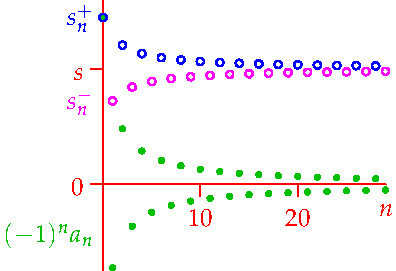
\includegraphics[scale=0.98]{alternatingharmonic}
\end{minipage}
\medbreak

The \emph{alternating} $\pm$-signs give the series its name. For us, however, the behavior of the sequence $(s_n)$ of partial sums is more interesting. Consider two subsequences $(\textcolor{blue}{s_n^+})=(s_{2n})$ and $(\textcolor{magenta}{s_n^-})=(s_{2n-1})$:
\begin{gather*}
	\textcolor{blue}{s_n^+}=\sum_{k=0}^{2n}(-1)^ka_k 
		 =1 -\biggl(\underbrace{\frac 12-\frac 13}_{a_1-a_2}\biggr) -\biggl(\underbrace{\frac 12-\frac 13}_{a_3-a_4}\biggr)-\cdots -\biggl(\underbrace{\frac 1{2n}-\frac 1{2n+1}}_{a_{2n-1}-a_{2n}}\biggr) \tag{$n\ge 0$}\\
	\textcolor{magenta}{s_n^-}=\sum_{k=0}^{2n-1}(-1)^ka_k =\biggl(\underbrace{1-\frac 12}_{a_0-a_1}\biggr) +\biggl(\underbrace{\frac 13-\frac 14}_{a_2-a_3}\biggr) +\cdots +\biggl(\underbrace{\frac 1{2n-1}-\frac 1{2n}}_{a_{2n-2}-a_{2n-1}}\biggr) \tag{$n\ge 1$}
\end{gather*}
Since the brackets are non-negative, $(s_n^+)$ is \textcolor{blue}{monotone-down} and $(s_n^-)$ \textcolor{magenta}{monotone-up.} Moreover,
\[\frac 12=\textcolor{magenta}{s_1^-}\le \textcolor{magenta}{s_n^-}\le \textcolor{magenta}{s_n^-}+a_{2n} = \textcolor{blue}{s_n^+} \le \textcolor{blue}{s_0^+} =1 \tag{$\dag$}\]
from which both subsequences are \emph{bounded} and thus \emph{convergent.} Not only this, but
\[\lim\bigl(\textcolor{blue}{s_n^+} -\textcolor{magenta}{s_n^-}\bigr) =\lim a_{2n} =0\]
shows that the limits of both subsequences are \emph{identical} (of course both are $s$).\goodbreak

The above discussion depended only on two simple properties of the sequence $(a_n)$; we've therefore proved a general statement.

\begin{thm}{Alternating series test}{}
	Let $(a_n)$ be monotone-down with $\lim a_n=0$.
	\begin{enumerate}
	  \item The series $\sum (-1)^na_n$ converges.
		\item If $(s_n)$ is the sequence of partial sums converging to $s=\sum (-1)^na_n$, then $\nm{s-s_n}\le a_{n+1}$.
	\end{enumerate} 
\end{thm}

Think about where our assumptions on $(a_n)$ are used in the proof. It can, in fact, be shown that the alternating harmonic series converges to $\ln 2$, although the estimates provided by the alternating series test make this a terrible method of approximation. Even summing the first 100 terms only results in 2 decimal places of accuracy!

\begin{examples}{}{}
	\exstart Since $a_n=\frac 1{n!}$ converges monotone-down to zero, the alternating series $\sum\frac{(-1)^{n+1}}{n!}$ converges. By taking the first 9 and 10 terms of this series, we see that
	\[0.9010498898\ldots\le\sum_{n=1}^\infty\frac{(-1)^{n+1}}{n!}\le 0.90105016538\ldots\]
	which at least yields the estimate $0.9015$ to 5 decimal places. The alternating series test is not required for this example, since it in fact converges absolutely.
	\begin{enumerate}\setcounter{enumi}{1}
	  \item The series $\sum_{n=2}^\infty\frac{\sin\frac\pi 2n}{\ln n}$ can be viewed as an alternating series since every \emph{even} term is zero. Writing $m=2n+1$, we obtain
	  \[
	  	\sum_{n=2}^\infty\frac{\sin\frac\pi 2n}{\ln n} =\sum_{m=1}^\infty\frac{\sin(\pi m+\frac\pi 2)}{\ln(2m+1)}= \sum_{m=1}^\infty\frac{(-1)^{m}}{\ln(2m+1)} 
	  \]
	  Since $\frac 1{\ln(2m+1)}$ decreases to zero, the alternating series test shows convergence.
	\end{enumerate}
\end{examples}

\medskip

\boldsubsubsection{Rearranging Infinite Series}

A \emph{rearrangement} of an infinite series $\sum a_n$ arises when we change the order of the terms of the sequence $(a_n)$ \emph{before} computing the sequence of partial sums. We still have to use every term $a_n$ in the new series. Since the resulting sequence of partials sums is likely completely different, we shouldn't assume that the new series has the same convergence properties as the old.

% The definition of an infinite series $\sum a_n$ requires that we compute partial sums
% \[s_n=a_1+\cdots +a_n\]
% by adding the terms $a_n$ in the order provided. 
% A \emph{rearrangement} of an infinite series means that we first change the order of the original sequence before computing partial sums. 

\begin{example}{}{riemannrearrangement}
	We rearrange the alternating harmonic series by summing \textcolor{blue}{two positive terms} before each \textcolor{magenta}{negative term}:
	\[
% 		\textcolor{blue}{a_1+a_3}+\textcolor{magenta}{a_2} +\textcolor{blue}{a_5+a_7}+\textcolor{magenta}{a_4} +\textcolor{blue}{a_9+a_{11}}+\textcolor{magenta}{a_6} +\cdots +\textcolor{blue}{a_{4n+1}+a_{4n+3}}+\textcolor{magenta}{a_{2n}} +\cdots
% 		
		\textcolor{blue}{1}+\textcolor{blue}{\frac 13} -\textcolor{magenta}{\frac 12} +\textcolor{blue}{\frac 15} +\textcolor{blue}{\frac 17} -\textcolor{magenta}{\frac 14} +\textcolor{blue}{\frac 19} +\textcolor{blue}{\frac 1{11}} -\textcolor{magenta}{\frac 16}  +\cdots +\textcolor{blue}{\frac 1{4n-3}} +\textcolor{blue}{\frac 1{4n-1}} -\textcolor{magenta}{\frac 1{2n}} +\cdots
	\]
	Every term in the original sequence is used here, so this is a genuine rearrangement. It is perhaps surprising to discover that the new series converges, though its limit is \emph{not the same} as the original alternating harmonic series! We leave the details to Exercise \ref{exs:riemannrearrangement}.
\end{example}

This behavior is quite different to that of finite sums, where the order of summation makes no difference at all. The situation can be summarized in a famous result of Riemann.

\begin{thm}{Riemann rearrangement}{}
	\exstart If $\sum a_n$ is conditionally convergent and $s\in\R\cup\{\pm\infty\}$, then there exists a rearrangement of the series which tends\footnotemark{} to $s$.
\begin{enumerate}\setcounter{enumi}{1}
  \item If $\sum a_n$ converges absolutely, then all rearrangements converge to the same limit.
\end{enumerate}
\end{thm}

\footnotetext{Riemann's result is in fact even stronger. Rearrangements also exist which diverge by oscillation between any given $\liminf$ and $\limsup$!}

The second part says that absolutely convergent series behave just like finite sums! We omit the proofs since they are lengthy and require nasty notation. Instead we illustrate the rough idea of part 1 via an example.

\begin{example}{}{riemannrearrange}
We show how to construct a rearrangement of the alternating harmonic series which converges to $s=\sqrt 2-1=0.41421\ldots$\smallbreak
First we convince ourselves that the sum of the positive terms $\sum a_n^+$ diverges to infinity. In this case the comparison test comes to our rescue:
\[\frac 1{2n-1}>\frac 1{2n}\implies \sum a_n^+=\sum \frac 1{2n-1}>\frac 12\sum \frac 1n=\infty\]
The negative terms also diverge $\sum a_n^-=-\infty$. Construction of the rearrangement is inductive.
\begin{enumerate}
  \item Sum just enough positive terms until the partial sum exceeds $s$: plainly $S_1=1$ will do.
	\item Sum negative terms starting at the beginning of the sequence until the sum is less than $s$:
	\[S_2=\textcolor{blue}{1}-\textcolor{magenta}{\frac 12}-\textcolor{magenta}{\frac 14}=0.25<s\]
	\item Repeat: add positive terms until the sum just exceeds $s$, then add negative terms, etc.,
	\begin{gather*}
	S_3=S_2+\textcolor{blue}{\frac 13}=0.583\ldots>s,\qquad S_4=S_3 -\textcolor{magenta}{\frac 16} -\textcolor{magenta}{\frac 18}=0.291\ldots<s
	\end{gather*}
\end{enumerate}
Continuing the process ad infinitum, we claim that
\[
	s=\textcolor{blue}{1}-\textcolor{magenta}{\frac 12}-\textcolor{magenta}{\frac 14} +\textcolor{blue}{\frac 13} -\textcolor{magenta}{\frac 16} -\textcolor{magenta}{\frac 18} +\textcolor{blue}{\frac 15} -\textcolor{magenta}{\frac 1{10}} +\textcolor{blue}{\frac 17}  -\textcolor{magenta}{\frac 1{12}}  -\textcolor{magenta}{\frac 1{14}} +\textcolor{blue}{\frac 19} -\textcolor{magenta}{\frac 1{16}} -\textcolor{magenta}{\frac 1{18}} +\textcolor{blue}{\frac 1{11}}  -\textcolor{magenta}{\frac 1{20}} +\textcolor{blue}{\frac 1{13}} -\cdots 
\]
To see why, observe:
\begin{itemize}
  \item Since $\sum a_n^+=\infty$ and $\sum a_n^-=-\infty$, at each stage we only add/subtract \emph{finitely many terms.}
  \item All terms of the original sequence $(a_n)$ are eventually used since we add the positive (negative) terms \emph{in order.} E.g., $a_{495}=\frac 1{495}$ appears, \emph{at the latest,} during the 495\th{} positive-addition phase.
  \item $\nm{S_n-s}\le \nm{a_{m_n}}$, where $a_{m_n}$ is the last term used at the $n\th$ stage. This plainly converges to zero, whence $\lim S_n=s$. 
\end{itemize}
\end{example}


% \begin{lemm}{}{}
% If $\sum a_n$ converges conditionally, then the sum of the positive terms diverges to $\infty$ and the negative terms to $-\infty$.
% \end{lemm}
% 
% \begin{proof}
% FALSE!!!
% Let $\sum^+a_n$ and $\sum^-a_n$ be these sub-series. If $\sum^+$ converges, then $\sum a_n-\sum^+a_n=\sum^-a_n$ converges, and so $\sum \nm{a_n}=\sum^+a_n-\sum^-a_n$ would converge. Contradiction. 
% \end{proof}
% 
% \begin{thm}{}{}
% \exstart If $\sum a_n$ is conditionally convergent and $s\in\R\cup\{\pm\infty\}$, then there exists a rearrangement of the series which tends to $s$.
% \begin{enumerate}\setcounter{enumi}{1}
%   \item If $\sum a_n$ is absolutely convergent, then any rearrangement of the terms of the series converges to the same thing.
% \end{enumerate}
% \end{thm}
% 
% \begin{proof}
% \begin{enumerate}
%   \item Let $s\in\R$ be given. Since $\sum^+a_n=\infty$, we may sum several terms (or none if $s<0$) starting at the beginning of the series such that the partial sum $S_{n_1}>s$.\par
%   Since $\sum^-a_n=-\infty$, we may now start adding negative terms in the series, again starting at the beginning, until the partial sum $S_{n_1+n_2}<s$.\par
%   Repeat this process ad infinitum. Observe:
%   \begin{itemize}
%     \item All terms in the series are used eventually since we are taking terms starting at the beginning of the sequence. For instance, if $a_n$ is the 495\th{} positive term in the sequence, then it will be added into our sum \emph{at the latest} by the 495\th{} positive contribution.
%     \item The resulting sequence of partial sums really does converge to $s$: this is since $\lim a_n=0$. This requires a little more proof. Given $\epsilon>0$, $\exists N$ such that $n>N\implies \nm{a_n}<\epsilon$. Suppose $S_{n_1+\cdots+n_k}<s$ and that we add $a_p+a_{p+1}+\cdots+a_{p+t}$ until we obtain $S_{n_1+\cdots +n_{k+1}}>s$. Plainly $\nm{S-s}<a_{p+t}\to 0$.
%   \end{itemize}
%   If $s=\infty$, the cheap proof is to take all the positive terms first. Alternatively, take positive terms until $S_{n_1}>1$, add the first negative term, then add more positive terms until $S_{n_1+n_2}>2$, and repeat. Plainly $S_{n_1+\cdots+n_k}>k\to \infty$ and this process uses up all terms in the series. The argument for $-\infty$ is similar.
%   
%   \item ??????
% \end{enumerate}
% \end{proof}




\begin{exercisessec}{}{}
	\exstart %[4.] and others
	Use the integral test to determine whether the series $\sum\limits_{n=1}^\infty\frac 1{n^2+1}$ converges or diverges.\vspace{-5pt}

\begin{enumerate}\setcounter{enumi}{1}  
  \item Prove Corollary \ref{cor:pseries} regarding the convergence/divergence of $p$-series.
  
  \item Let $\smash{s_n=\sum\limits_{k=1}^n\frac 1{\sqrt k}}$. Estimate how many terms are required before $s_n\ge 100$.

	\item (Example \ref*{ex:inttestex}.\ref{ex:integralsuperslow}) Verify the claim that $\smash{\sum\limits_{n=2}^\infty\frac 1{n\ln n}=\infty}$. If you want a challenge, verify the estimate claim also.
%    \item Determine whether $\sum \frac 1{n\ln n\ln\ln n}$ converges or diverges.

  
%   \item\begin{enumerate}
%     \item Use calculus to show that $a_n=\frac{\ln n}{n^2}$ is monotone-down whenever $n\ge 2$.
%     \item Show that $\lim a_n=0$, and that the hypotheses of the integral test are therefore satisfied.\par
%     (\emph{Hint: You may use without proof that $\ln n<n$ for large $n$})
%     \item Determine whether the series $\sum_{n=2}^\infty\frac{\ln n}{n^2}$ converges or diverges.
%   \end{enumerate}
  
  \item\begin{enumerate}
    \item %[6a]
    Give an example of a series $\sum a_n$ which converges, but for which $\sum a_n^2$ diverges.\par
		(\emph{Exercise \ref*{sec:series}.\ref{exs:seriesmult} really requires that $\sum a_n$ be absolutely convergent!})
		\item Give an example of a divergent series $\sum b_n$ for which $\sum b_n^2$ converges.
  \end{enumerate}
  
  
  \item Suppose $(a_n)$ satisfies the hypotheses of the alternating series test \emph{except} that $\lim a_n=a>0$. What can you say about the sequences $(s_n^+)$ and $(s_n^-)$ and the series $\sum (-1)^na_n$?
  
  
  \item\label{exs:integralestimates}
%   \begin{enumerate}
%         \item Suppose $f(x)$ and $(a_n)$ satisfy the hypotheses of the integral test. Prove that, for any $m\ge 2$,
% 		\[\int_{m}^{n+1}f(x)\,\dx\le\sum_{k=m}^n a_k\le \int_{m-1}^nf(x)\,\dx\]
		%\item	
		We know that the harmonic series has a growth rate comparable to $\ln n$. Let $a_n=\frac 1n$ and define a new sequence $(t_n)$ by
		\[t_n=s_n-\ln n =1+\frac 12+\cdots +\frac 1n-\ln n\]
		where $s_n=\sum\limits_{k=1}^na_n$ is the $n\th$ partial sum. Prove that $(t_n)$ is a positive, monotone-down sequence, which therefore converges.\footnotemark{}\par
		(\emph{Hint: you'll need the mean value theorem from elementary calculus})
	%\end{enumerate}

	
  \item\begin{enumerate}
    \item Show that the series $\sum\limits_{n=1}^\infty \frac{(-1)^nn}{n^2+1}$ is conditionally convergent to some real number $s$.
    \item How many terms are required for the partial sum $s_n$ to approximate $s$ to within $0.01$.
    \item Following Example \ref{ex:riemannrearrange}, use a calculator to state the first 15 terms in a rearrangement of the series in part (a) which converges to 0. 
  \end{enumerate} 
	
	\item\label{exs:riemannrearrangement} In Example \ref{ex:riemannrearrangement} we rearranged the terms of the alternating harmonic series by taking two positive terms before each negative term.
	\begin{enumerate}
	  \item Verify, for each $n\in\N$, that
		\[
			b_n:=\frac 1{4n-3}+\frac 1{4n-1}-\frac 1{2n}>0
		\]
		whence the \emph{subsequence} of partial sums $(s_{3n})$ is monotone-up.
		\item Use the comparison test to show that $\sum b_n$ converges.
		\item Prove that the rearranged series converges, to some value $s>\frac 56$.\par
		(\emph{Thus $s>\ln 2\approx 0.69$, the limit of the original alternating harmonic series})
	\end{enumerate}
		
\end{enumerate}
\end{exercisessec}

\vspace{-5pt}

\footnotetext{The limit $\gamma:=\lim t_n\approx 0.5772$ is the \emph{Euler--Mascheroni constant.} It appears in many mathematical identities, and yet very little about it is known; it is not even known whether $\gamma$ is irrational!}